\documentclass[svgnames,table,,aspectratio=169]{beamer}
%\documentclass[svgnames,table,handout,aspectratio=129]{beamer}
\usepackage{hhline}
\usepackage{etoolbox}
\usepackage{tikz}
\usepackage{mathtools}
\usepackage{amssymb}
%\usepackage{/usr/lib64/R/share/texmf/Sweave}
\usepackage{polynom}
\usepackage{qrcode}


%\input{latexdefinitions}
\definecolor{georgiaRed}{RGB}{100,0,00}
\definecolor{mediumGray}{gray}{0.6}



\usetheme{Frankfurt}%
%\usetheme{Warsaw}%
%\useoutertheme{smoothbars}


%\usecolortheme{seagull}
\usecolortheme{beaver}
\logo{\includegraphics[height=.125in]{ugaLogo}}

% Note that the colour definitions are given in the latexDefinitions
% file.
\setbeamercolor{palette primary}{fg=georgiaRed,bg=white}
\setbeamercolor{palette secondary}{fg=georgiaRed,bg=white}
\setbeamercolor{palette tertiary}{fg=georgiaRed,bg=white}
\setbeamercolor{palette quaternary}{bg=mediumGray,fg=black}
\setbeamercolor{block title}{fg=white,bg=georgiaRed}
\setbeamercolor{block body}{fg=black,bg=black!10}
\setbeamercolor{titlelike}{bg=georgiaRed,fg=white} % parent=palette quaternary}

% Define the variable to determine whether or not the clicker quizzes
% are visible in the resulting output.
\newtoggle{clicker}
\toggletrue{clicker}
%\togglefalse{clicker}


% To display a lecture uncomment out the "includeonly" line below to
% match the name of the file. You do not have to do anything with the
% lecture line below and can leave it commented out. It is in place
% because at one time we had multiple lectures within a file, but that
% has been changed.



\mode<presentation>{
  \setbeamercovered{invisible}
  \setbeameroption{hide notes}
}

\mode<handout>{
 
  \usepackage{pgfpages}
  %\pgfpagesuselayout{4 on 1}[letterpaper, border shrink=5mm]
  \pgfpagesuselayout{resize to}[letterpaper,border shrink=5mm]
  \setbeameroption{show notes}


  %\pgfpagesphysicalpageoptions{logical pages=2,physical
  %height=\pgfpageoptionheight,physical width=\pgfpageoptionwidth}
  % Set up the pages for notes.
  % This idea and some code came from
  % http://www.guidodiepen.nl/2009/07/creating-latex-beamer-handouts-with-notes/



  \pgfpagesdeclarelayout{3 on 1 with notes} {
    \edef\pgfpageoptionheight{11in} %\the\paperheight}
    \edef\pgfpageoptionwidth{8.5in} %\the\paperwidth}
    \edef\pgfpageoptionborder{0pt}
  }

  {

	\AtBeginDocument{
      \newbox\notesbox
      \setbox\notesbox=\vbox{
        \hsize=\paperwidth
        \vskip-2.5cm\hskip-5cm\vbox{
          \textcolor{light-gray}{\hrule width 12.6cm\vskip0.5cm}
          \textcolor{light-gray}{\hrule width 12.6cm\vskip0.5cm}
          \textcolor{light-gray}{\hrule width 12.6cm\vskip0.5cm}
          \textcolor{light-gray}{\hrule width 12.6cm\vskip0.5cm}
          \textcolor{light-gray}{\hrule width 12.6cm\vskip0.5cm}
          \textcolor{light-gray}{\hrule width 12.6cm\vskip0.5cm}
          \textcolor{light-gray}{\hrule width 12.6cm\vskip0.5cm}
          \textcolor{light-gray}{\hrule width 12.6cm\vskip0.5cm}
          \textcolor{light-gray}{\hrule width 12.6cm\vskip0.5cm}
          \textcolor{light-gray}{\hrule width 12.6cm\vskip0.5cm}
          \textcolor{light-gray}{\hrule width 12.6cm\vskip0.5cm}
          \textcolor{light-gray}{\hrule width 12.6cm\vskip0.5cm}
          \textcolor{light-gray}{\hrule width 12.6cm\vskip0.5cm}
          \textcolor{light-gray}{\hrule width 12.6cm\vskip0.5cm}
          \textcolor{light-gray}{\hrule width 12.6cm\vskip0.5cm}
          \textcolor{light-gray}{\hrule width 12.6cm\vskip0.5cm}
          \textcolor{light-gray}{\hrule width 12.6cm\vskip0.5cm}
          \textcolor{light-gray}{\hrule width 12.6cm\vskip0.5cm}
          \textcolor{light-gray}{\hrule width 12.6cm\vskip0.5cm}

          \vspace*{-9.75cm}
          \textcolor{light-gray}{\rule[-1.0cm]{1pt}{9.25cm}\hskip0.5cm}
          \textcolor{light-gray}{\rule[-1.0cm]{1pt}{9.25cm}\hskip0.5cm}
          \textcolor{light-gray}{\rule[-1.0cm]{1pt}{9.25cm}\hskip0.5cm}
          \textcolor{light-gray}{\rule[-1.0cm]{1pt}{9.25cm}\hskip0.5cm}
          \textcolor{light-gray}{\rule[-1.0cm]{1pt}{9.25cm}\hskip0.5cm}
          \textcolor{light-gray}{\rule[-1.0cm]{1pt}{9.25cm}\hskip0.5cm}
          \textcolor{light-gray}{\rule[-1.0cm]{1pt}{9.25cm}\hskip0.5cm}
          \textcolor{light-gray}{\rule[-1.0cm]{1pt}{9.25cm}\hskip0.5cm}
          \textcolor{light-gray}{\rule[-1.0cm]{1pt}{9.25cm}\hskip0.5cm}
          \textcolor{light-gray}{\rule[-1.0cm]{1pt}{9.25cm}\hskip0.5cm}
          \textcolor{light-gray}{\rule[-1.0cm]{1pt}{9.25cm}\hskip0.5cm}
          \textcolor{light-gray}{\rule[-1.0cm]{1pt}{9.25cm}\hskip0.5cm}
          \textcolor{light-gray}{\rule[-1.0cm]{1pt}{9.25cm}\hskip0.5cm}
          \textcolor{light-gray}{\rule[-1.0cm]{1pt}{9.25cm}\hskip0.5cm}
          \textcolor{light-gray}{\rule[-1.0cm]{1pt}{9.25cm}\hskip0.5cm}
          \textcolor{light-gray}{\rule[-1.0cm]{1pt}{9.25cm}\hskip0.5cm}
          \textcolor{light-gray}{\rule[-1.0cm]{1pt}{9.25cm}\hskip0.5cm}
          \textcolor{light-gray}{\rule[-1.0cm]{1pt}{9.25cm}\hskip0.5cm}
          \textcolor{light-gray}{\rule[-1.0cm]{1pt}{9.25cm}\hskip0.5cm}
          \textcolor{light-gray}{\rule[-1.0cm]{1pt}{9.25cm}\hskip0.5cm}

        }

      }

    \pgfpagesphysicalpageoptions
    {%
      logical pages=6,%
      physical height=\pgfpageoptionheight,%
      physical width=\pgfpageoptionwidth,%
      last logical shipout=3%
    }
    
    \pgfpageslogicalpageoptions{1}
    {%
      border shrink=\pgfpageoptionborder,%
      resized width=.5\pgfphysicalwidth,%
      resized height=.33\pgfphysicalheight,%
      center=\pgfpoint{.25\pgfphysicalwidth}{.82\pgfphysicalheight}%
    }%
    \pgfpageslogicalpageoptions{2}
    {%
      border shrink=\pgfpageoptionborder,%
      resized width=.5\pgfphysicalwidth,%
      resized height=.33\pgfphysicalheight,%
      center=\pgfpoint{.25\pgfphysicalwidth}{.47\pgfphysicalheight}%
    }%
    \pgfpageslogicalpageoptions{3}
    {%
      border shrink=\pgfpageoptionborder,%
      resized width=.5\pgfphysicalwidth,%
      resized height=.33\pgfphysicalheight,%
      center=\pgfpoint{.25\pgfphysicalwidth}{.17\pgfphysicalheight}%
    }%	
	\pgfpageslogicalpageoptions{4}
    {%
      border shrink=\pgfpageoptionborder,%
      resized width=.5\pgfphysicalwidth,%
      resized height=.33\pgfphysicalheight,%
      center=\pgfpoint{.85\pgfphysicalwidth}{.82\pgfphysicalheight},%
      copy from=4
    }%
    \pgfpageslogicalpageoptions{5}
    {%
      border shrink=\pgfpageoptionborder,%
      resized width=.5\pgfphysicalwidth,%
      resized height=.33\pgfphysicalheight,%
      center=\pgfpoint{.85\pgfphysicalwidth}{.47\pgfphysicalheight},%
      copy from=5
    }%
    \pgfpageslogicalpageoptions{6}
    {%
      border shrink=\pgfpageoptionborder,%
      resized width=.5\pgfphysicalwidth,%
      resized height=.33\pgfphysicalheight,%
      center=\pgfpoint{.85\pgfphysicalwidth}{.17\pgfphysicalheight},%
      copy from=6
    }%
    
      \pgfpagesshipoutlogicalpage{4}\copy\notesbox
      \pgfpagesshipoutlogicalpage{5}\copy\notesbox
      \pgfpagesshipoutlogicalpage{6}\copy\notesbox
    }
  }

  \pgfpagesuselayout{3 on 1 with notes}

}

\setbeamercolor{upper separation line head}{bg=red}
\setbeamercolor{headline}{bg=red}
\setbeamertemplate{headline}
{%
\begin{beamercolorbox}{section in head/foot}
\insertsectionnavigationhorizontal{.75\textwidth}{}{}
\hfill \insertpagenumber /\insertdocumentendpage
\end{beamercolorbox}%
}
\setbeamercolor{section number projected}{bg=red,fg=black}
\setbeamercolor{subsection number projected}{bg=red,fg=black}
%\setbeamercolor{frametitle}{bg=lightgray,fg=black}

\setbeamertemplate{itemize item}{\color{georgiaRed}$\blacklozenge$}
\setbeamertemplate{itemize subitem}{\color{georgiaRed}$\blacktriangleright$}

\newcommand{\dotfield}[2]{%
  \begin{tikzpicture}[y=0.25cm, x=0.25cm,font=\sffamily]
    \foreach \y in {0,...,#2} {
      \foreach \x in {0,...,#1} {
        \draw[fill=georgiaRed,opacity=0.1] (\x,\y)  circle [radius=0.03em];
      }
    }
  \end{tikzpicture}
}

\newcommand{\twoByTwo}[4]{%
  \left[
    \begin{array}{rr}
      #1 & #2 \\
      #3 & #4 \\
    \end{array}
  \right]
}

\newcommand{\threeByThree}[9]{%
  \left[
    \begin{array}{rrr}
      #1 & #2 & #3 \\
      #4 & #5 & #6 \\
      #7 & #8 & #9
    \end{array}
  \right]
}

\newcommand{\columnVector}[1]{%
  \left[
    \begin{array}{r}
    #1                           
    \end{array}
  \right]
}


\begin{document}



\author{\textsc{T. Alli$^{a}$, K. Black$^{a}$}}
\institute{$^a$Department of Mathematics, University of Georgia, GA}
\subject{Linear Algebra}
\keywords{Linear Transformation, Vectors, Matrices, Linear Algebra}

%\lecture{Partial Fractions}{partial-fractions}
%\section{Rational Functions}

\title{Section 3.2: One-To-One and Onto Transformations}
\subtitle{The Relationship Between The Domain And Range}


\date{} % {\today}

\begin{frame}
  \titlepage
\end{frame}

\begin{frame}{Outline}
  \tableofcontents
\end{frame}


\section{Goals}

\begin{frame}{Goals}

  \begin{itemize}
  \item Determine if a transformation is one-to-one or not one-to-one.
  \item Determine if a transformation is onto or not onto.
  \item Use the reduced row echelon form (RREF) of a matrix to
    determine if a transformation is one-to-one or if it is onto.
  \end{itemize}

\end{frame}

\section{One-to-one Transformations}

\begin{frame}{Example: one dimension}
  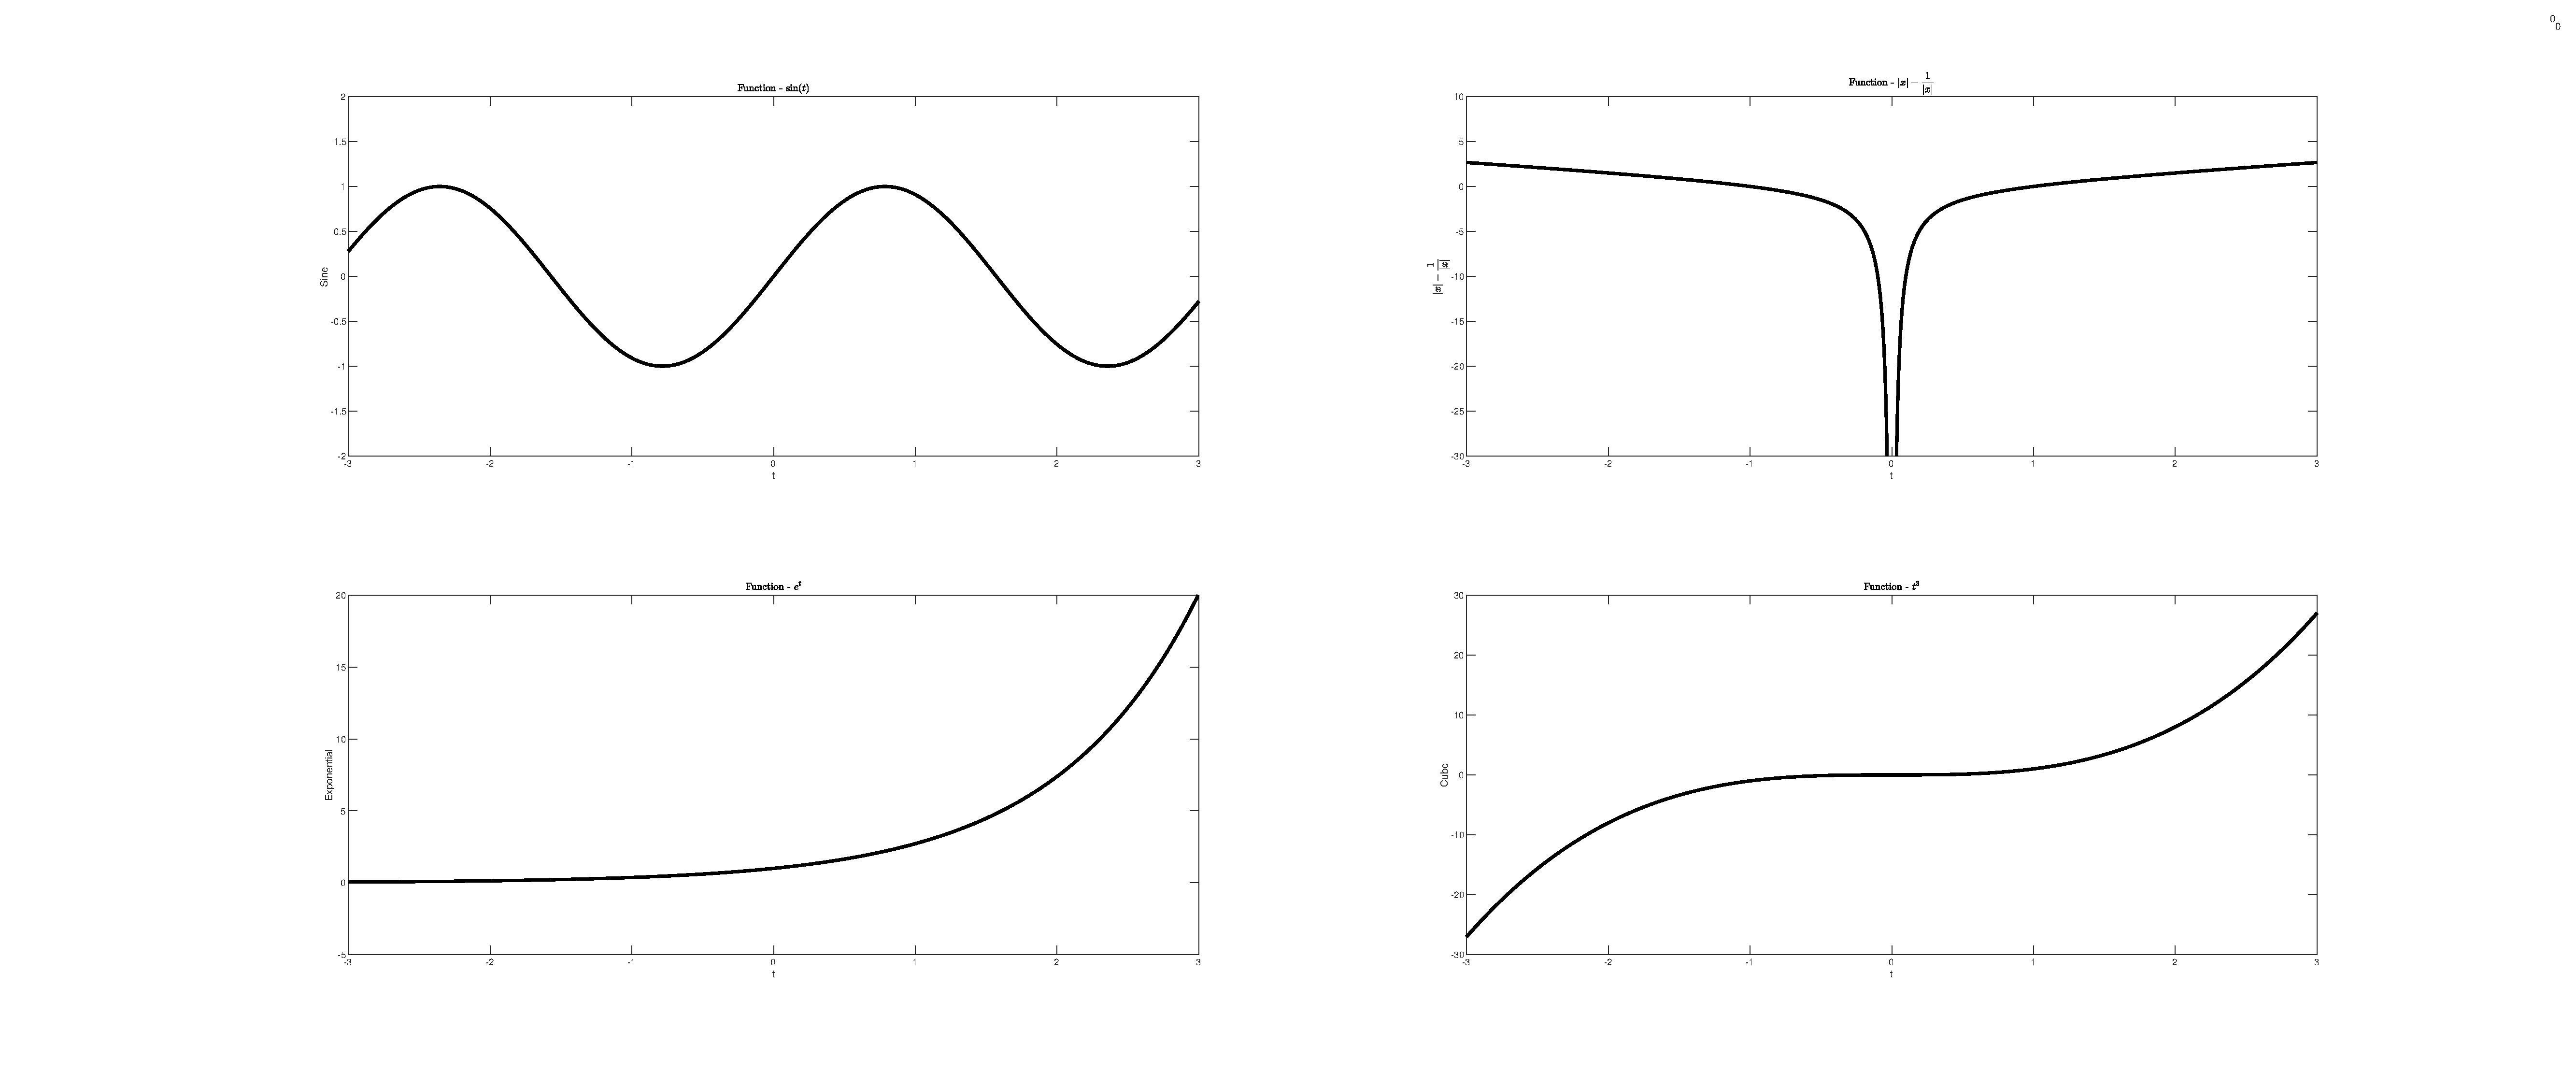
\includegraphics[width=\textwidth]{oneDFunctions.pdf}
\end{frame}

\begin{frame}{Example: Linear Transformation}

  \begin{align*}
    T: &  {\mathbb R}^2  \rightarrow  {\mathbb R}^2, & \\
    T\vec{x} & = \twoByTwo{1}{1}{1}{-1} \columnVector{x \\ y}
       & = x \columnVector{1\\1} + y \columnVector{1\\-1}.
  \end{align*}

  \dotfield{60}{24}
    
\end{frame}

\begin{frame}{Example: Linear Transformation}

  \begin{align*}
    T: &  {\mathbb R}^3  \rightarrow  {\mathbb R}^2, & \\
    T\vec{x} & =
               \left[
               \begin{array}{rrr}
                 1 & 3 & 4 \\
                 2 & 4 & 6
               \end{array}
               \right]
               \columnVector{x \\ y \\ z}
       & = x \columnVector{1\\2} + y \columnVector{3\\4} + z \columnVector{4\\6}.
  \end{align*}

  \dotfield{60}{24}
    
\end{frame}

\begin{frame}{Example: Linear Transformation}

  \begin{align*}
    T: &  {\mathbb R}^2  \rightarrow  {\mathbb R}^3, & \\
    T\vec{x} & =
               \left[
               \begin{array}{rr}
                  1 &  3 \\
                  2 &  6 \\
                 -1 & -3 
               \end{array}
               \right]
               \columnVector{x \\ y }
       & = x \columnVector{1\\2\\-1} + y \columnVector{3\\6\\-3}.
  \end{align*}

  \dotfield{60}{24}
    
\end{frame}

\begin{frame}{One-To-One Transformation}

  \begin{block}{Definition: One-To-One Transformation}
    A transformation,
    \begin{eqnarray*}
      T: {\mathbb R}^n \rightarrow {\mathbb R}^m,
    \end{eqnarray*}
    is \textbf{one-to-one} if for every $\vec{b}$ in the
    \textit{range} of the transformation, there is \textit{exactly
      one} $\vec{x}$ in the domain of the transformation where
    $T\left(\vec{x}\right)=\vec{b}$.
  \end{block}

  \uncover<2->{
    \begin{itemize}
    \item Given any vector $\vec{b}$ in ${\mathbb R}^m$ there is
      either one or zero solutions to the equation $
      T\left(\vec{x}\right)=\vec{b}$.
    \item If $T\left(\vec{u}\right)=T\left(\vec{v}\right)$ then
      $\vec{u}=\vec{v}$.
    \item If $T\left(\vec{u}\right)\neq T\left(\vec{v}\right)$ then
      $\vec{u}\neq\vec{v}$.
    \end{itemize}
  }
  
\end{frame}

\begin{frame}{So What?}

  Suppose that a transformation is one-to-one...
  \begin{itemize}
  \item Given any vector $\vec{b}$ in ${\mathbb R}^m$ there is
    either one or zero solutions to the equation $
    T\left(\vec{x}\right)=\vec{b}$.
  \item If $T\left(\vec{u}\right)=T\left(\vec{v}\right)$ then
    $\vec{u}=\vec{v}$.
  \item If $T\left(\vec{u}\right)\neq T\left(\vec{v}\right)$ then
    $\vec{u}\neq\vec{v}$.
  \end{itemize}

  \dotfield{60}{24}

  % properties
  % Ax=b has either one solution or no solutions.
  % Ax=0 is only true if x=0
  % The columns of A are linearly independent.
  % A has a pivot in every column.
  % range of T has dimension n
  
\end{frame}

\begin{frame}{Example}

  \begin{align*}
    T: &  {\mathbb R}^2  \rightarrow  {\mathbb R}^3, & \\
    T\vec{x} & =
               \left[
               \begin{array}{rr}
                  2 & -2 \\
                  1 &  4 \\
                 -1 &  1
               \end{array}
               \right]
               \columnVector{a \\ b}
       & = a \columnVector{2\\1\\-1} + b \columnVector{-2\\4\\1}.
  \end{align*}

  \dotfield{60}{24}
  
\end{frame}


\section{Onto Transformations}


\begin{frame}{Onto Transformations}

  \begin{block}{Definition: Onto Transformation}
    A transformation,
    \begin{eqnarray*}
      T: {\mathbb R}^n \rightarrow {\mathbb R}^m,
    \end{eqnarray*}
    is \textbf{onto} if for \textit{every} $\vec{b}$ in
    ${\mathbb R}^m$, there is \textit{at least one} $\vec{x}$ in the
    domain of the transformation where
    $T\left(\vec{x}\right)=\vec{b}$.
  \end{block}

  \uncover<2->{
    \begin{itemize}
    \item The range of the transformation is ${\mathbb R}^m$.
    \item Given any vector in ${\mathbb R}^m$ you can find at least
      one solution to $T\left(\vec{x}\right)=\vec{b}$.
    \end{itemize}
  }
  
\end{frame}

\begin{frame}{So What?}

  Suppose that a transformation is onto....
  \begin{itemize}
  \item We can always find one or more solutions to
    $T\left(\vec{x}\right)=\vec{b}$.
  \end{itemize}

  \dotfield{60}{24}

  % properties
  % Ax=b is consistent for every b in R^m (There are 1 or inf. solutions.)
  % The columns of A span R^m
  % A has a pivot in every row
  
\end{frame}


\begin{frame}{Example: Linear Transformation}

  \begin{align*}
    T: &  {\mathbb R}^2  \rightarrow  {\mathbb R}^2, & \\
    T\vec{x} & = \twoByTwo{1}{1}{2}{-1} \columnVector{x \\ y}
       & = x \columnVector{1\\2} + y \columnVector{1\\-1}.
  \end{align*}

  \dotfield{60}{24}
    
\end{frame}

\begin{frame}{Example: Linear Transformation}

  \begin{align*}
    T: &  {\mathbb R}^3  \rightarrow  {\mathbb R}^2, & \\
    T\vec{x} & =
               \left[
               \begin{array}{rrr}
                  2 & 4 & -2 \\
                  1 & 1 &  1 \\
               \end{array}
               \right]
               \columnVector{x \\ y \\\ z} 
       & = x \columnVector{2\\1} + y \columnVector{4\\1} +
           z\columnVector{-2 \\ 1}.
  \end{align*}

  \dotfield{60}{24}
    
\end{frame}


\begin{frame}{Blank Page}
  \dotfield{60}{24}
\end{frame}


\end{document}
